% Options for packages loaded elsewhere
% Options for packages loaded elsewhere
\PassOptionsToPackage{unicode}{hyperref}
\PassOptionsToPackage{hyphens}{url}
\PassOptionsToPackage{dvipsnames,svgnames,x11names}{xcolor}
%
\documentclass[
  11pt,
]{article}
\usepackage{xcolor}
\usepackage[margin=1in]{geometry}
\usepackage{amsmath,amssymb}
\setcounter{secnumdepth}{5}
\usepackage{iftex}
\ifPDFTeX
  \usepackage[T1]{fontenc}
  \usepackage[utf8]{inputenc}
  \usepackage{textcomp} % provide euro and other symbols
\else % if luatex or xetex
  \usepackage{unicode-math} % this also loads fontspec
  \defaultfontfeatures{Scale=MatchLowercase}
  \defaultfontfeatures[\rmfamily]{Ligatures=TeX,Scale=1}
\fi
\usepackage{lmodern}
\ifPDFTeX\else
  % xetex/luatex font selection
\fi
% Use upquote if available, for straight quotes in verbatim environments
\IfFileExists{upquote.sty}{\usepackage{upquote}}{}
\IfFileExists{microtype.sty}{% use microtype if available
  \usepackage[]{microtype}
  \UseMicrotypeSet[protrusion]{basicmath} % disable protrusion for tt fonts
}{}
\usepackage{setspace}
\makeatletter
\@ifundefined{KOMAClassName}{% if non-KOMA class
  \IfFileExists{parskip.sty}{%
    \usepackage{parskip}
  }{% else
    \setlength{\parindent}{0pt}
    \setlength{\parskip}{6pt plus 2pt minus 1pt}}
}{% if KOMA class
  \KOMAoptions{parskip=half}}
\makeatother
% Make \paragraph and \subparagraph free-standing
\makeatletter
\ifx\paragraph\undefined\else
  \let\oldparagraph\paragraph
  \renewcommand{\paragraph}{
    \@ifstar
      \xxxParagraphStar
      \xxxParagraphNoStar
  }
  \newcommand{\xxxParagraphStar}[1]{\oldparagraph*{#1}\mbox{}}
  \newcommand{\xxxParagraphNoStar}[1]{\oldparagraph{#1}\mbox{}}
\fi
\ifx\subparagraph\undefined\else
  \let\oldsubparagraph\subparagraph
  \renewcommand{\subparagraph}{
    \@ifstar
      \xxxSubParagraphStar
      \xxxSubParagraphNoStar
  }
  \newcommand{\xxxSubParagraphStar}[1]{\oldsubparagraph*{#1}\mbox{}}
  \newcommand{\xxxSubParagraphNoStar}[1]{\oldsubparagraph{#1}\mbox{}}
\fi
\makeatother


\usepackage{longtable,booktabs,array}
\usepackage{calc} % for calculating minipage widths
% Correct order of tables after \paragraph or \subparagraph
\usepackage{etoolbox}
\makeatletter
\patchcmd\longtable{\par}{\if@noskipsec\mbox{}\fi\par}{}{}
\makeatother
% Allow footnotes in longtable head/foot
\IfFileExists{footnotehyper.sty}{\usepackage{footnotehyper}}{\usepackage{footnote}}
\makesavenoteenv{longtable}
\usepackage{graphicx}
\makeatletter
\newsavebox\pandoc@box
\newcommand*\pandocbounded[1]{% scales image to fit in text height/width
  \sbox\pandoc@box{#1}%
  \Gscale@div\@tempa{\textheight}{\dimexpr\ht\pandoc@box+\dp\pandoc@box\relax}%
  \Gscale@div\@tempb{\linewidth}{\wd\pandoc@box}%
  \ifdim\@tempb\p@<\@tempa\p@\let\@tempa\@tempb\fi% select the smaller of both
  \ifdim\@tempa\p@<\p@\scalebox{\@tempa}{\usebox\pandoc@box}%
  \else\usebox{\pandoc@box}%
  \fi%
}
% Set default figure placement to htbp
\def\fps@figure{htbp}
\makeatother





\setlength{\emergencystretch}{3em} % prevent overfull lines

\providecommand{\tightlist}{%
  \setlength{\itemsep}{0pt}\setlength{\parskip}{0pt}}



 
\usepackage[]{biblatex}
\addbibresource{references.bib}


\usepackage{hyperref}
\hypersetup{
  colorlinks=true,
  linkcolor=blue,
  urlcolor=blue,
  breaklinks=true,
  pdfborder={0 0 0}
}
\makeatletter
\@ifpackageloaded{caption}{}{\usepackage{caption}}
\AtBeginDocument{%
\ifdefined\contentsname
  \renewcommand*\contentsname{Table of contents}
\else
  \newcommand\contentsname{Table of contents}
\fi
\ifdefined\listfigurename
  \renewcommand*\listfigurename{List of Figures}
\else
  \newcommand\listfigurename{List of Figures}
\fi
\ifdefined\listtablename
  \renewcommand*\listtablename{List of Tables}
\else
  \newcommand\listtablename{List of Tables}
\fi
\ifdefined\figurename
  \renewcommand*\figurename{Figure}
\else
  \newcommand\figurename{Figure}
\fi
\ifdefined\tablename
  \renewcommand*\tablename{Table}
\else
  \newcommand\tablename{Table}
\fi
}
\@ifpackageloaded{float}{}{\usepackage{float}}
\floatstyle{ruled}
\@ifundefined{c@chapter}{\newfloat{codelisting}{h}{lop}}{\newfloat{codelisting}{h}{lop}[chapter]}
\floatname{codelisting}{Listing}
\newcommand*\listoflistings{\listof{codelisting}{List of Listings}}
\makeatother
\makeatletter
\makeatother
\makeatletter
\@ifpackageloaded{caption}{}{\usepackage{caption}}
\@ifpackageloaded{subcaption}{}{\usepackage{subcaption}}
\makeatother
\usepackage{bookmark}
\IfFileExists{xurl.sty}{\usepackage{xurl}}{} % add URL line breaks if available
\urlstyle{same}
\hypersetup{
  pdftitle={William's Update},
  pdfauthor={William Clinton Co},
  colorlinks=true,
  linkcolor={blue},
  filecolor={Maroon},
  citecolor={blue},
  urlcolor={blue},
  pdfcreator={LaTeX via pandoc}}


\title{William's Update}
\usepackage{etoolbox}
\makeatletter
\providecommand{\subtitle}[1]{% add subtitle to \maketitle
  \apptocmd{\@title}{\par {\large #1 \par}}{}{}
}
\makeatother
\subtitle{Remittances}
\author{William Clinton Co}
\date{August 12, 2025}
\begin{document}
\maketitle
\begin{abstract}
This report provides a review of available remittance datasets and
literature. The analysis identifies the World Bank as the primary data
source, offering both cost of remittances data (detailed,
corridor-level) and remittance flows data (aggregate, less frequent
updates). Key findings indicate that remittance datasets are generally
limited in scope and quality, with bilateral flows being estimated
rather than directly observed. The report evaluates supplementary
sources including RemitScope. A literature review categorizes relevant
research by geographic focus and methodological approach. The report
concludes that while the World Bank provides the most comprehensive
global coverage, data access remains challenging and researchers often
rely on estimated rather than actual transaction data.
\end{abstract}

\renewcommand*\contentsname{Table of contents}
{
\hypersetup{linkcolor=}
\setcounter{tocdepth}{10}
\tableofcontents
}

\setstretch{1}
\section{Introduction}\label{introduction}

Remittance datasets are generally limited in scope and quality. This
report presents the best available datasets and summarizes key
literature on remittance measurement. Most research focuses on the
effects of remittances rather than forecasting flows. There are two main
types of datasets: cost of remittances (detailed, corridor-level) and
actual remittance flows (often less accurate and updated infrequently).
The World Bank provides the primary source for both, with most other
datasets derived from their data. Remitscope is also worth mentioning as
a potential dataset, given its completeness. More details can be found
in the \hyperref[remitscope]{Remitscope section}.

\section{Best Dataset: World Bank}\label{best-dataset-world-bank}

\subsection{Cost of Remittances
Dataset}\label{cost-of-remittances-dataset}

This is a more comprehensive dataset. Please see the
\href{https://github.com/WilliamClintC/RER/blob/main/data/Remittance_2/rpw_dataset_2011_2024_q3.xlsx}{sample
dataset} where we can observe source and destination countries.

We can also observe the firm, payment instrument (bank transfer, cash,
etc.), and speed.

There are many different methodologies with regards to remittances. For
an overview, please see the
\href{https://remittanceprices.worldbank.org/resources}{World Bank's
resources page}.

The World Bank aims to establish \emph{unified standards and maintain
public data availability}. See
\href{https://remittanceprices.worldbank.org/national-and-regional-databases-certified-by-the-world-bank}{certified
national and regional databases}. There are issues with their data
request site; I have submitted several requests without receiving
instructions. The dataset should be available at:
\href{https://remittanceprices.worldbank.org/file-download/remittance-prices-worldwide-2011-2024q3-dataset}{World
Bank Remittance Prices Dataset}.

\subsection{Remittances Flows Dataset}\label{remittances-flows-dataset}

The following fields are available:

\begin{figure}[H]

{\centering \pandocbounded{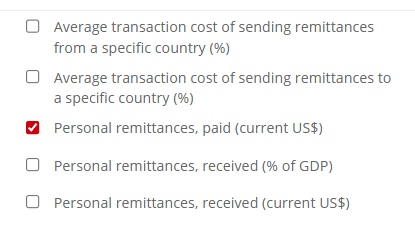
\includegraphics[keepaspectratio]{images/Screenshot 2025-08-07 063601.png}}

}

\caption{Available Fields for Remittances Sent Dataset}

\end{figure}%

Bilateral remittance flows are not directly observable; only aggregate
data is available. The corridor-level dataset is released infrequently.
According to the literature:

\begin{quote}
Additionally, the World Bank also publishes estimates on bilateral
remittance flows. The basis for bilateral remittances estimates are
weighted migrant stock data, the weighted income of migrants based on
the per capita income in the country of destination, and the weighted
income in the origin country of the migrant (Ratha and Shaw, 2007: 43).
\end{quote}

The main dataset is available at:
\href{https://databank.worldbank.org/metadataglossary/world-development-indicators/series/BM.TRF.PWKR.CD.DT}{World
Bank Development Indicators - Personal Remittances}. See limitations at
the
\href{https://databank.worldbank.org/metadataglossary/world-development-indicators/series/BM.TRF.PWKR.CD.DT}{metadata
page}.

\begin{quote}
Because direct measurement (tracking actual transactions) is often
incomplete, they use a mix of methods: direct reporting when possible
and estimates/models to fill in gaps.
\end{quote}

\subsubsection{Derivative Datasets}\label{derivative-datasets}

\begin{enumerate}
\def\labelenumi{\arabic{enumi}.}
\tightlist
\item
  \href{https://www.migrationdataportal.org/data-catalogue}{Migration
  Data Portal}
\item
  \href{https://unctadstat.unctad.org/datacentre/reportInfo/US.Remittances}{UNCTAD
  Statistics - US Remittances}
\item
  \href{https://www.migrationpolicy.org/programs/data-hub/global-remittances-guide}{Migration
  Policy Institute - Global Remittances Guide}

  \begin{itemize}
  \tightlist
  \item
    \href{https://www.migrationpolicy.org/programs/data-hub/charts/total-remittance-inflows-and-outflows-1980-present?width=1000&height=850&iframe=true}{Total
    Remittance Inflows and Outflows (1980-Present)}
  \item
    \href{https://www.migrationpolicy.org/programs/data-hub/charts/remittance-trends-over-time?width=1000&height=850&iframe=true}{Remittance
    Trends Over Time}
  \item
    \href{https://www.migrationpolicy.org/programs/data-hub/charts/bilateral-remittance-flows?width=1000&height=850&iframe=true}{Bilateral
    Remittance Flows}
  \end{itemize}
\item
  \href{https://data.worldbank.org/indicator/bx.trf.pwkr.cd.dt}{World
  Bank - Personal Remittances Received}
\item
  \href{https://data.adb.org/taxonomy/term/130}{Asian Development Bank -
  Remittances Data}
\end{enumerate}

\subsection{Remitscope}\label{remitscope}

Consider \href{https://remitscope.org/latin-america/themes/}{RemitScope}
as an additional resource. See the
\href{https://remitscope.org/how-to-use-remitscope/}{guide} for usage.
RemitScope aggregates data from various sources, including bilateral
flows, but these are not always easily accessible.

\begin{quote}
RemitSCOPE brings together data from secondary sources, that are usually
scattered in different organisations and agencies, as well as collecting
data through primary research and directly from market operators and
regulators.
\end{quote}

Currently, RemitScope covers Africa and Latin America. Asia is coming
soon.

\begin{figure}[H]

{\centering \pandocbounded{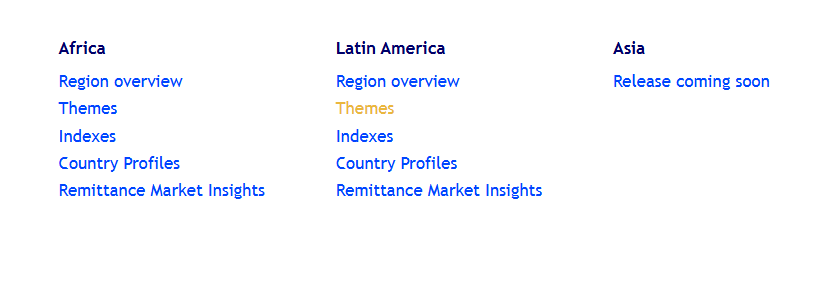
\includegraphics[keepaspectratio]{images/Screenshot 2025-08-11 005134.png}}

}

\caption{RemitScope Regional Coverage}

\end{figure}%

See the
\href{https://remitscope.org/wp-content/uploads/2023/08/RemitSCOPE-Thematic-Dashboards-Overview.pdf}{RemitSCOPE
Thematic Dashboards Overview}:

\begin{figure}[H]

{\centering \pandocbounded{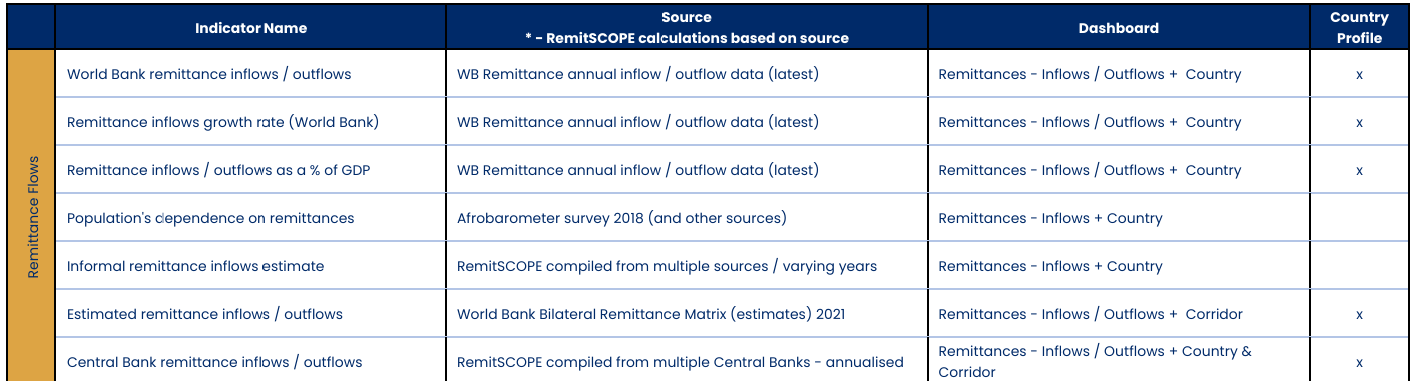
\includegraphics[keepaspectratio]{images/Screenshot 2025-08-11 010105.png}}

}

\caption{RemitSCOPE Dataset Overview}

\end{figure}%

RemitScope provides visualization tools; data scraping may be required
for analysis.

\begin{figure}[H]

{\centering \pandocbounded{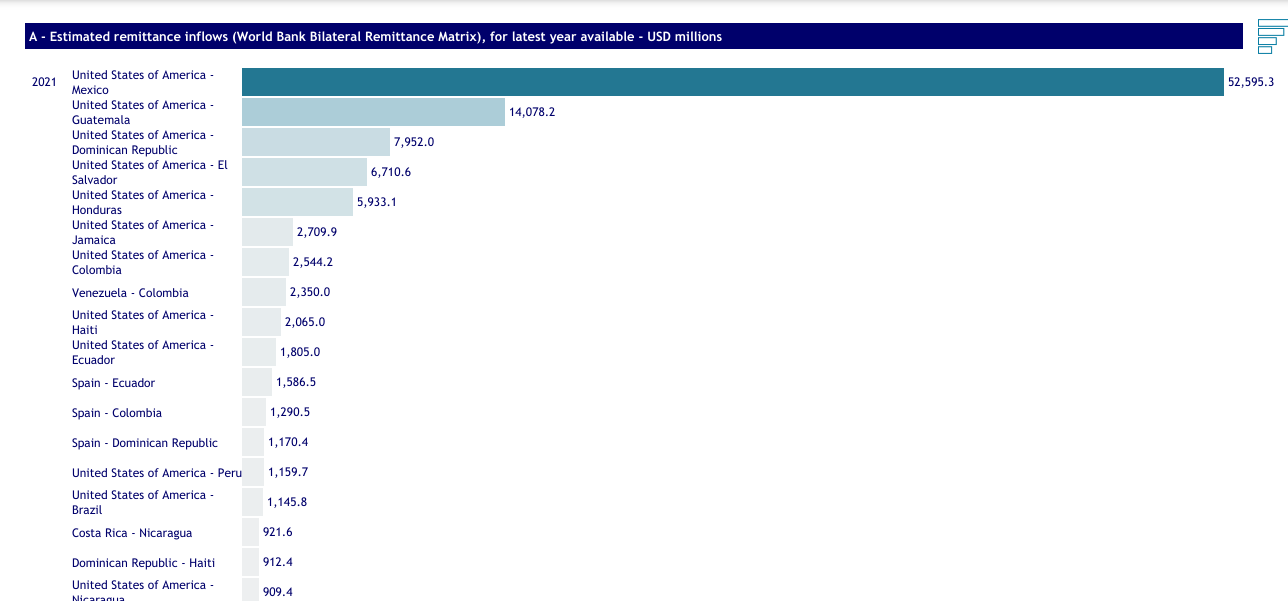
\includegraphics[keepaspectratio]{images/Screenshot 2025-08-11 014421.png}}

}

\caption{RemitScope Example Visualization}

\end{figure}%

Explore more at
\href{https://remitscope.org/latin-america/themes/}{RemitScope Latin
America Themes}.

\subsection{Canadian International Development Platform:
CIDP}\label{canadian-international-development-platform-cidp}

The \href{https://cidpnsi.ca/remittances-explorer/}{CIDP Remittances
Explorer} uses World Bank datasets to create interactive remittance data
visualizations. The dataset is available for download from the project
repository:
\href{https://github.com/WilliamClintC/RER/blob/main/data/Remittance_2/CIDP.csv}{CIDP
Remittances Data}

\subsection{Additional Data Sources}\label{additional-data-sources}

\begin{itemize}
\tightlist
\item
  \href{https://sdgstoday.org/dataset/remittances}{SDGs Today
  Remittances Dataset} - Sustainable Development Goals tracking platform
  for remittance data
\end{itemize}

\subsection{Data Request Status}\label{data-request-status}

\subsection{World Bank}\label{world-bank}

I have submitted a data request through the
\href{https://remittanceprices.worldbank.org/data-download}{World Bank's
data download portal} for the most current and comprehensive remittance
datasets.

\subsection{Wise \& Remitly}\label{wise-remitly}

I contacted Remitly and Wise to request data access. Wise denied our
request:

\begin{figure}[H]

{\centering \pandocbounded{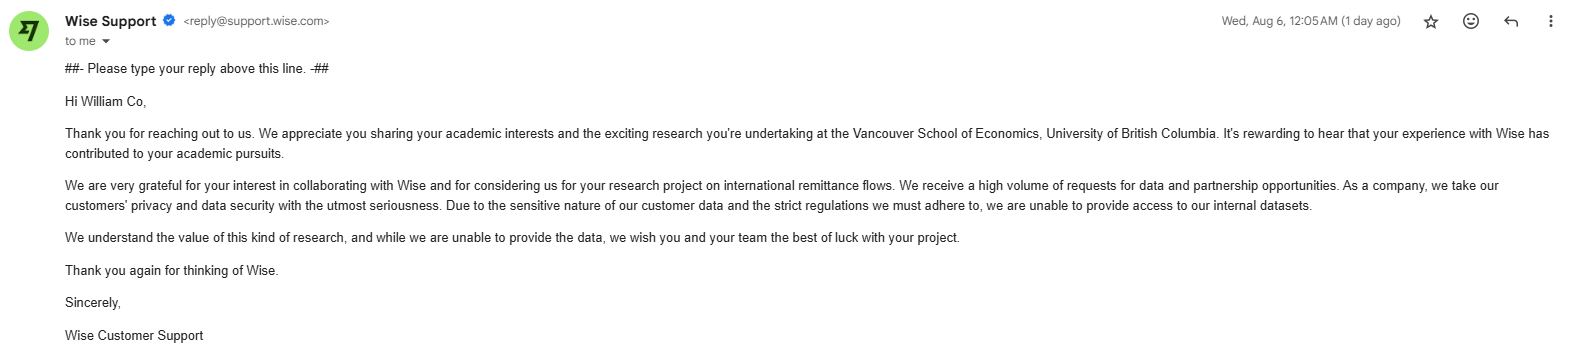
\includegraphics[keepaspectratio]{images/Screenshot 2025-08-07 153221.png}}

}

\caption{Wise Data Request Rejection}

\end{figure}%

\section{Literature Review}\label{literature-review}

\subsection{High Relevance}\label{high-relevance}

\subsubsection{Country/Region Case
Studies}\label{countryregion-case-studies}

\paragraph{\texorpdfstring{\href{https://www.elibrary.imf.org/view/journals/001/2022/203/article-A001-en.xml}{The
Propensity to Remit: Macro and Micro Factors Driving Remittances to
Central America and the
Caribbean}}{The Propensity to Remit: Macro and Micro Factors Driving Remittances to Central America and the Caribbean}}\label{the-propensity-to-remit-macro-and-micro-factors-driving-remittances-to-central-america-and-the-caribbean}

\textbf{Authors:} Hussein Bidawi, Paola Aliperti F. Domingues, Chiara
Fratto, Nicole Laframboise\\
\textbf{Publication Date:} 2022\\
\textbf{Comment:} Promising paper (we have corridor-level data
(Remitscope)) for Latin American countries.

\paragraph{\texorpdfstring{\href{https://www.aercafrica.org/publications/research-papers/macroeconomic-determinants-of-remittance-flows-to-sub-saharan-africa/}{Macroeconomic
Determinants of Remittance Flows to Sub-Saharan
Africa}}{Macroeconomic Determinants of Remittance Flows to Sub-Saharan Africa}}\label{macroeconomic-determinants-of-remittance-flows-to-sub-saharan-africa}

\textbf{Authors:} Deodat E. Adenutsi, Christian R. K. Ahortor\\
\textbf{Publication Date:} 2021\\
\textbf{Comment:} Focuses on Sub-Saharan Africa.

\paragraph{\texorpdfstring{\href{https://www.elibrary.imf.org/view/journals/001/2009/216/article-A001-en.xml}{Determinants
and Macroeconomic Impact of Remittances in Sub-Saharan
Africa}}{Determinants and Macroeconomic Impact of Remittances in Sub-Saharan Africa}}\label{determinants-and-macroeconomic-impact-of-remittances-in-sub-saharan-africa}

\textbf{Authors:} Raju J Singh, Kyung-woo Lee, Markus Haacker\\
\textbf{Publication Date:} 2009\\
\textbf{Comment:} IMF paper, slightly older.

\paragraph{\texorpdfstring{\href{https://www.elibrary.imf.org/view/journals/001/2011/018/article-A001-en.xml?ArticleTabs=Related\%20Documents}{Determinants
of Remittances: Evidence From
Tonga}}{Determinants of Remittances: Evidence From Tonga}}\label{determinants-of-remittances-evidence-from-tonga}

\textbf{Author:} Huidan Lin\\
\textbf{Publication Date:} 2011\\
\textbf{Comment:} Focuses on Tonga.

\paragraph{\texorpdfstring{\href{https://www.imf.org/en/Publications/WP/Issues/2016/12/31/Macroeconomic-Determinants-of-Remittances-Evidence-from-India-18728}{Macroeconomic
Determinants of Remittances: Evidence from
India}}{Macroeconomic Determinants of Remittances: Evidence from India}}\label{macroeconomic-determinants-of-remittances-evidence-from-india}

\textbf{Author:} Poonam Gupta\\
\textbf{Publication Date:} 2005\\
\textbf{Comment:} Relevant but dated.

\subsubsection{\texorpdfstring{\href{https://cepr.org/voxeu/columns/defying-odds-remittances-held-during-covid-19-pandemic}{Defying
the Odds: Remittances Held Up During the COVID-19
Pandemic}}{Defying the Odds: Remittances Held Up During the COVID-19 Pandemic}}\label{defying-the-odds-remittances-held-up-during-the-covid-19-pandemic}

\textbf{Working Paper:}
\href{https://www.imf.org/en/Publications/WP/Issues/2021/07/16/Defying-the-Odds-Remittances-During-the-COVID-19-Pandemic-461321}{IMF
Working Paper}\\
\textbf{Authors:} Saad Quayyum, Kangni Kpodar, Montfort Mlachila,
Vigninou Gammadigbe\\
\textbf{Publication Date:} 2021\\
\textbf{Comment:} Uses COVID-19 as a ``shock'' to analyze remittances.

\subsubsection{\texorpdfstring{\href{https://cepr.org/voxeu/columns/remittances-and-vulnerability-developing-countries-results-new-dataset-remittances}{Remittances
and Vulnerability in Developing Countries: Results from a New Dataset on
Remittances from
Italy}}{Remittances and Vulnerability in Developing Countries: Results from a New Dataset on Remittances from Italy}}\label{remittances-and-vulnerability-in-developing-countries-results-from-a-new-dataset-on-remittances-from-italy}

\textbf{Authors:} Andrea Presbitero, Nikola Spatafora, Giulia Bettin\\
\textbf{Publication Date:} 2014\\
\textbf{Comment:} Focuses on Italy.

\subsubsection{\texorpdfstring{\href{https://www.elibrary.imf.org/view/journals/001/2022/087/article-A001-en.xml}{What
Explains Remittance Fees? Panel
Evidence}}{What Explains Remittance Fees? Panel Evidence}}\label{what-explains-remittance-fees-panel-evidence}

\textbf{Authors:} Thorsten Beck, Mathilde Janfils, Kangni R Kpodar\\
\textbf{Publication Date:} 2022\\
\textbf{Comment:} IMF paper on remittance fees.

\subsubsection{\texorpdfstring{\href{https://pmc.ncbi.nlm.nih.gov/articles/PMC9510564/pdf/10290_2022_Article_478.pdf}{Monetary
Policy and Remittance Flows in Latin America and the
Caribbean}}{Monetary Policy and Remittance Flows in Latin America and the Caribbean}}\label{monetary-policy-and-remittance-flows-in-latin-america-and-the-caribbean}

\textbf{Publication Date:} 2022\\
\textbf{Comment:} Examines monetary policy and remittance flows in Latin
America and the Caribbean.

\subsection{Medium Relevance}\label{medium-relevance}

\subsubsection{\texorpdfstring{\href{https://www.sciencedirect.com/science/article/pii/S0313592620304094}{Determinants
of International Remittance Inflow in Asia-Pacific Middle-Income
Countries}}{Determinants of International Remittance Inflow in Asia-Pacific Middle-Income Countries}}\label{determinants-of-international-remittance-inflow-in-asia-pacific-middle-income-countries}

\textbf{Authors:} Naoyuki Yoshino, Farhad Taghizadeh-Hesary, Miyu
Otsuka\\
\textbf{Publication Date:} 2020\\
\textbf{Comment:} Directly relevant, but not as academically reputable
as high relevance papers.

\subsubsection{\texorpdfstring{\href{https://drive.google.com/file/d/1e893ibGZcECt9gxIpPgq2XEE2kDGgqx-/view?usp=sharing}{Migrant
Remittances}}{Migrant Remittances}}\label{migrant-remittances}

\textbf{Author:} Dean Yang\\
\textbf{Publication Date:} 2011\\
\textbf{Comment:} Highly regarded, but dated.

\subsubsection{\texorpdfstring{\href{https://academic.oup.com/wber/article/21/2/219/1701529}{Are
Remittances Insurance? Evidence from Rainfall Shocks in the
Philippines}}{Are Remittances Insurance? Evidence from Rainfall Shocks in the Philippines}}\label{are-remittances-insurance-evidence-from-rainfall-shocks-in-the-philippines}

\textbf{Authors:} Dean Yang, HwaJung Choi\\
\textbf{Publication Date:} 2007\\
\textbf{Comment:} Uses rainfall shocks to analyze remittance
determinants.

\subsubsection{\texorpdfstring{\href{https://www.statcan.gc.ca/en/catalogue/11-008-X201100211619}{Remittance
Behaviours Among Recent Immigrants in
Canada}}{Remittance Behaviours Among Recent Immigrants in Canada}}\label{remittance-behaviours-among-recent-immigrants-in-canada}

\textbf{Publication Date:} 2011\\
\textbf{Comment:} Statistics Canada paper on remittance behaviour in
Canada.

\subsubsection{\texorpdfstring{\href{https://www.econstor.eu/handle/10419/204586}{Migrant
Remittances: Alternative Money Transfer
Channels}}{Migrant Remittances: Alternative Money Transfer Channels}}\label{migrant-remittances-alternative-money-transfer-channels}

\textbf{Authors:} Martina Metzger, Tim Riedler, Jennifer Pédussel Wu\\
\textbf{Publication Date:} 2019\\
\textbf{Comment:} Explores remittance transfer channels.

\subsubsection{\texorpdfstring{\href{https://documents1.worldbank.org/curated/en/701621468149081927/pdf/693130PUB0publ067926B09780821388266.pdf}{Migration
and Remittances during the Global Financial Crisis and
Beyond}}{Migration and Remittances during the Global Financial Crisis and Beyond}}\label{migration-and-remittances-during-the-global-financial-crisis-and-beyond}

\textbf{Editors:} Dilip Ratha, Jeffrey H. Cohen, Ibrahim Sirkeci\\
\textbf{Publication Date:} 2012\\
\textbf{Comment:} World Bank book, somewhat dated.

\subsection{Low Relevance}\label{low-relevance}

\subsubsection{\texorpdfstring{\href{http://www.nber.org/papers/w12325}{International
Migration, Remittances, and Household Investment: Evidence from
Philippine Migrants' Exchange Rate
Shocks}}{International Migration, Remittances, and Household Investment: Evidence from Philippine Migrants' Exchange Rate Shocks}}\label{international-migration-remittances-and-household-investment-evidence-from-philippine-migrants-exchange-rate-shocks}

\textbf{Author:} Dean Yang\\
\textbf{Publication Date:} 2006\\
\textbf{Comment:} Relevant but old; analyzes currency appreciation as a
determinant of remittances.

\section{Appendix}\label{appendix}

Additional datasets used in academic research can be found at: -
\href{https://www.icpsr.umich.edu/web/ICPSR/search/studies?start=0&sort=score\%20desc\%2CTITLE_SORT\%20asc&ARCHIVE=ICPSR&PUBLISH_STATUS=PUBLISHED&rows=50&q=Remittances}{ICPSR
- Remittances Studies} -
\href{https://dataverse.harvard.edu/dataset.xhtml?persistentId=doi:10.7910/DVN/I6VB8V}{Harvard
Dataverse - Remittances Dataset} -
\href{https://dataverse.harvard.edu/dataset.xhtml?persistentId=doi:10.7910/DVN/SV0PIW}{Harvard
Dataverse - Additional Remittances Dataset}


\printbibliography



\end{document}
